
\documentclass{article}
\usepackage[T1]{fontenc}
\usepackage{graphicx}
\usepackage{amsmath, amsthm, amssymb}
\usepackage{hyperref}
\usepackage{polski}
\usepackage{listings}
\usepackage{color}
\usepackage{enumerate}
\usepackage{float}
\lstset{
	language=C++,
	basicstyle=\ttfamily\footnotesize,
	keywordstyle=\color{blue}\bfseries,
	commentstyle=\color{green},
	stringstyle=\color{red},
	numberstyle=\tiny\color{green},
	numbers=left,
	stepnumber=1,
	tabsize=4,
	breaklines=true,
	showstringspaces=false
}
\title{Raport AiSD lista 1}
\author{Amelia Dorożko}
\date{\today}
\begin{document}
	\maketitle
Do analizy poszczególnych algorytmów sortujących, bazowałam na przykładowo 8 wygenerowanych listach o zadanych długościach oraz elementach z zakresu od $0$ do $999$.
\section{Sortowanie przez wstawianie}
\subsection{\texttt{INSERTION\_SORT}}

W tej metodzie każda kolejna liczba z tablicy jest porównywana z elementami po jej lewej stronie i wstawiana na odpowiednie miejsce.
\begin{table}[h!]
	\centering
	\small
	\begin{tabular}{|c|c|c|}
		\hline
		\small
		\textbf{Długość tablicy (n)} & \textbf{Liczba porównań} & \textbf{Liczba przypisań} \\ \hline
		5   & 4     & 12     \\ \hline
		10  & 22    & 40     \\ \hline
		100 & 2615  & 2813   \\ \hline
		200 & 10045 & 10443  \\ \hline
		400 & 37341 & 38139  \\ \hline
		600 & 86800 & 87998  \\ \hline
		800 & 163804 & 165402 \\ \hline
		1000 & 249193 & 251191 \\ \hline
	\end{tabular}
	\caption{INSERTION\_SORT}
\end{table}
\subsection{\texttt{MODIFIED\_INSERTION\_SORT}}
Sortowanie przez wstawianie oraz jego zmodyfikowana wersja, jest algorytmem o złożoności czasowej \emph{O($n^2$)} w najgorszym z możliwych wypadków. 
\\ \texttt{MODIFIED\_INSERTION\_SORT}, gdy przesuwamy większy element, równocześnie "za darmo" przesuwamy też mniejszy element pary, który będzie potrzebował tej samej serii operacji. Główna pętla przechodzi przez listę co dwa indeksy, co zmniejsza liczbę iteracji pętli o połowę. Przy dużych tablicach ta zmiana znacznie obniża czas wykonania.
\begin{lstlisting}
void MODIFIED_INSERTION_SORT(int A[], int n) {
	for (int i = 1; i < n - 1; i += 2) {
		int pierwszy = A[i - 1];
		int drugi = A[i];
		liczbaPrzypisan += 2;
		if (pierwszy > drugi) {
			liczbaPorownan++;
			swap(pierwszy, drugi);
			liczbaPrzypisan += 2;
		}
		int j = i - 2;
		while (j >= 0 && A[j] > drugi) {
			liczbaPorownan++;
			A[j + 2] = A[j];
			liczbaPrzypisan++;
			j --;
		}
		A[j + 2] = drugi;
		while (j >= 0 && A[j] > pierwszy) {
			liczbaPorownan++;
			A[j + 1] = A[j];
			liczbaPrzypisan++;
			j --;
		}
		A[j + 1] = pierwszy;
		liczbaPrzypisan += 2;
		
	}
\end{lstlisting}
W celu uzyskania pełnej poprawności algorytmu, należało rozważyć przypadek dla tablic o nieparzystej ilości elementów,
\begin{lstlisting}
	if (n % 2!= 0) {
		liczbaPorownan++;
		int ostatni = A[n - 1];
		liczbaPrzypisan++;
		int j = n - 2;
		while (j >= 0 && A[j] > ostatni) {
			liczbaPorownan++;
			A[j + 1] = A[j];
			liczbaPrzypisan++;
			j--;
		}
		A[j + 1] = ostatni;
		liczbaPrzypisan++;
	}


\end{lstlisting}
\begin{table}[h!]
	\centering
	\small 
	\begin{tabular}{|c|c|c|}
		\hline
		\textbf{Długość tablicy (n)} & \textbf{Liczba porównań} & \textbf{Liczba przypisań} \\ \hline
		5   & 5     & 14     \\ \hline
		10  & 12   &   29   \\ \hline
		100 & 1606  & 1826   \\ \hline
		200 & 6666 & 7116  \\ \hline
		400 & 25417 & 26320  \\ \hline
		600 & 56965 & 58307  \\ \hline
		800 & 108414 & 110217 \\ \hline
		1000 & 164210 & 166450 \\ \hline
	\end{tabular}
	\caption{MODIFIED\_INSERTION\_SORT}
\end{table}



\section{Sortowanie przez scalanie}

\subsection{\texttt{MERGE\_SORT}}
Klasyczny \texttt{MERGE\_SORT} dzieli tablicę na dwie części, sortuje je rekurencyjnie, a następnie scala dwie posortowane części, co daje całkowitą złożoność \emph{O($n \log(n)$)}.


\begin{table}[h!]
	\centering
	\small
	\begin{tabular}{|c|c|c|}
		\hline
		\textbf{Długość tablicy (n)} & \textbf{Liczba porównań} & \textbf{Liczba przypisań} \\ \hline
		5   & 16    & 32     \\ \hline
		10  & 43    & 86     \\ \hline
		100 & 771   & 1542   \\ \hline
		200 & 1743  & 3486   \\ \hline
		400 & 3887  & 7774   \\ \hline
		600 & 6175  & 12350  \\ \hline
		800 & 8575  & 17150  \\ \hline
		1000 & 10975 & 21950  \\ \hline
	\end{tabular}
	\caption{MERGE\_SORT}
\end{table}

\subsection{\texttt{MODIFIED\_MERGE\_SORT}}
 W przypadku zmodyfikowanego \texttt{MERGE\_SORT}, dzielimy tablicę na trzy części zamiast dwóch. Mimo że scalanie trzech tablic wymaga więcej porównań, mniejsza liczba poziomów rekurencyjnych sprawia, że całkowity koszt operacji  może być niższy. Tutaj mamy więcej segmentów, co może prowadzić do lepszej wydajności, zwłaszcza dla dużych danych.

\begin{lstlisting}
int s1 = p + (k - p) / 3;
int s2 = p + 2 * (k - p) / 3; 
MODIFIED_MERGE_SORT(A, p, s1);
MODIFIED_MERGE_SORT(A, s1 + 1, s2);
MODIFIED_MERGE_SORT(A, s2 + 1, k);
MODIFIED_MERGE(A, p, s1, s2, k);
\end{lstlisting}
Również należy zwrócić uwagę poniższy fragment kodu:
\begin{lstlisting}
	L[n1] = INT_MAX;
	M[n2] = INT_MAX;
	P[n3] = INT_MAX;
\end{lstlisting}
Umożliwia on algorytmowi efektywne zakończenie procesu łączenia, gdy wszystkie elementy zostały już przetworzone.
\begin{table}[h!]
	\centering
	\small
	\begin{tabular}{|c|c|c|}
		\hline
		\textbf{Długość tablicy (n)} & \textbf{Liczba porównań} & \textbf{Liczba przypisań} \\ \hline
		5   & 12    & 27     \\ \hline
		10  & 27    & 59     \\ \hline
		100 & 497   & 1053   \\ \hline
		200 & 1121  & 2363   \\ \hline
		400 & 2592  & 5462   \\ \hline
		600 & 3964  & 8292   \\ \hline
		800 & 5377  & 11189  \\ \hline
		1000 & 7177  & 14989  \\ \hline
	\end{tabular}
	\caption{MODIFIED\_MERGE\_SORT}
\end{table}



\section{Sortowanie przez kopcowanie}

\subsection{\texttt{HEAP\_SORT}}
\texttt{HEAP\_SORT} tworzy kopiec binarny z tablicy, a następnie wielokrotnie usuwa największy element, który umieszcza na końcu tablicy, odbudowując kopiec dla pozostałych elementów, co łącznie daje złożoność \emph{O($n \log(n)$)}.

\begin{table}[h!]
	\centering
	\small
	\begin{tabular}{|c|c|c|}
		\hline
		\textbf{Długość tablicy (n)} & \textbf{Liczba porównań} & \textbf{Liczba przypisań} \\ \hline
		5   & 13    & 27     \\ \hline
		10  & 47    & 86     \\ \hline
		100 & 1146  & 1823   \\ \hline
		200 & 2828  & 4403   \\ \hline
		400 & 6608  & 10131  \\ \hline
		600 & 10740 & 16362  \\ \hline
		800 & 15132 & 22936  \\ \hline
		1000 & 19751 & 29817  \\ \hline
	\end{tabular}
	\caption{HEAP\_SORT}
\end{table}


\subsection{\texttt{MODIFIED\_HEAP\_SORT}}
Modyfikacja algorytmu \texttt{HEAP\_SORT} polega na wprowadzeniu kopca ternarnego.Mniejsza "głębokość" kopca oznacza, że operacje przesiewania \texttt{MODIFIED\_HEAPIFY} muszą być wykonywane rzadziej, ponieważ mniejsze jest "drzewo", które algorytm musi przetworzyć. Warto wyróżnić sposób modyfikacji funkcji \texttt{HEAPIFY}, która obsługuje dodatkowych potomków:
\begin{lstlisting}
	
	if (l < n && A[l] > A[largest])  {
		liczbaPorownan++;
		liczbaPrzypisan++;
		largest = l;
	}
	if (m < n && A[m] > A[largest]) {
		liczbaPorownan++;
		liczbaPrzypisan++;
		largest = m;
	}
	if (r < n && A[r] > A[largest]) {
		liczbaPorownan++;
		liczbaPrzypisan++;
		largest = r;
	}
	if (largest != i) {
		swap(A[i], A[largest]);
		liczbaPorownan++;
		liczbaPrzypisan += 2;
		MODIFIED_HEAPIFY(A, n, largest);
	}
\end{lstlisting}

\begin{table}[h!]
	\centering
	\begin{tabular}{|c|c|c|}
		\hline
		\small
		\textbf{Długość tablicy (n)} & \textbf{Liczba porównań} & \textbf{Liczba przypisań} \\ \hline
		5   & 10    & 22     \\ \hline
		10  & 32    & 63     \\ \hline
		100 & 849   & 1365   \\ \hline
		200 & 2039  & 3216   \\ \hline
		400 & 4655  & 7196   \\ \hline
		600 & 7728  & 11831  \\ \hline
		800 & 10903 & 16558  \\ \hline
		1000 & 14248 & 21504  \\ \hline
	\end{tabular}
	\caption{MODIFIED\_HEAP\_SORT}
	

\end{table}


\subsubsection*{Porównanie klasycznych i zmodyfikowanych algorytmów sortowania}

\begin{enumerate}
 \item Przyrównując obie wersje algorytmu \texttt{INSERTON\_MERGE}, po wprowadzeniu niewielkich zmian zauważamy, że zmodyfikowany algorytm jest znacznie wydatniejszy od swojej zwykłej wersji.
  \begin{figure}[H]
 	\centering
 	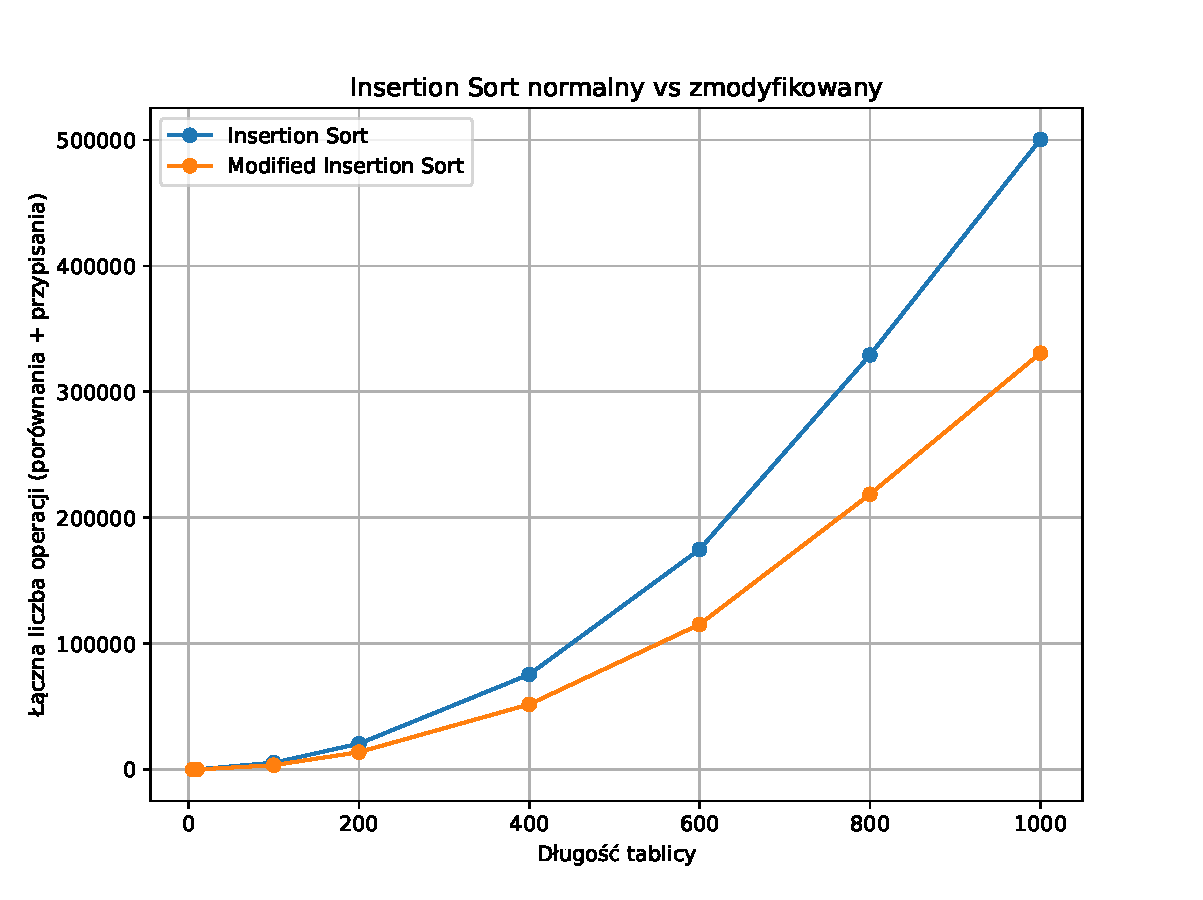
\includegraphics[width=1\textwidth]{Figure_1.1.pdf}
 \end{figure}
 \item Kolejne dwie wersje modyfikacji, są korzystniejszym rozwiązaniem.

 \begin{figure}[H]
 	\centering
 	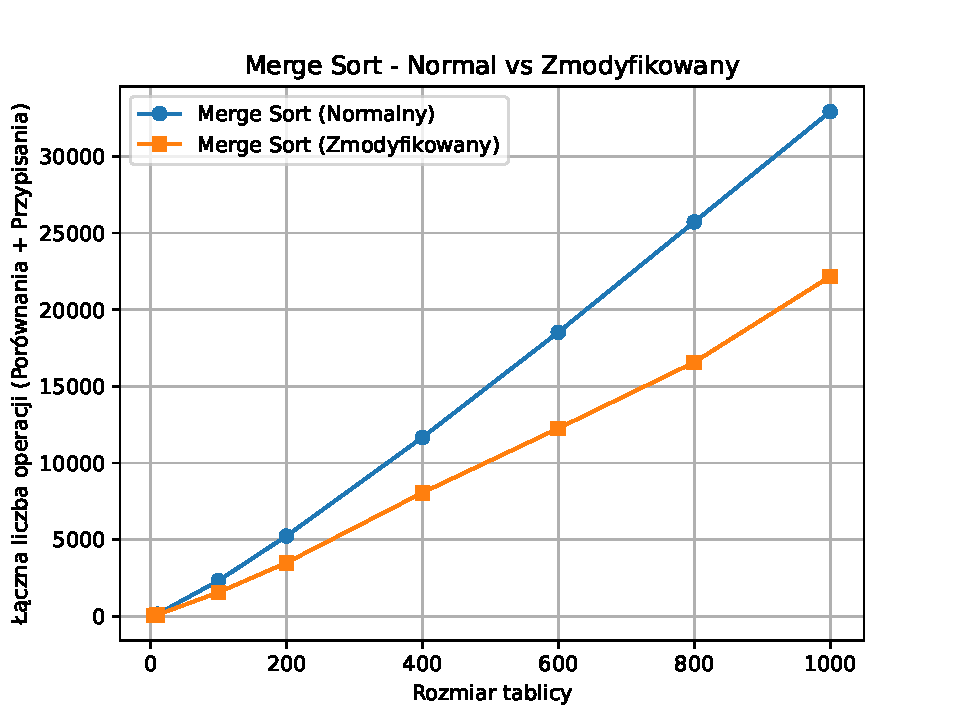
\includegraphics[width=1\textwidth]{Figure_2.pdf}
 \end{figure}
 \begin{figure}[H]
 	\centering
 	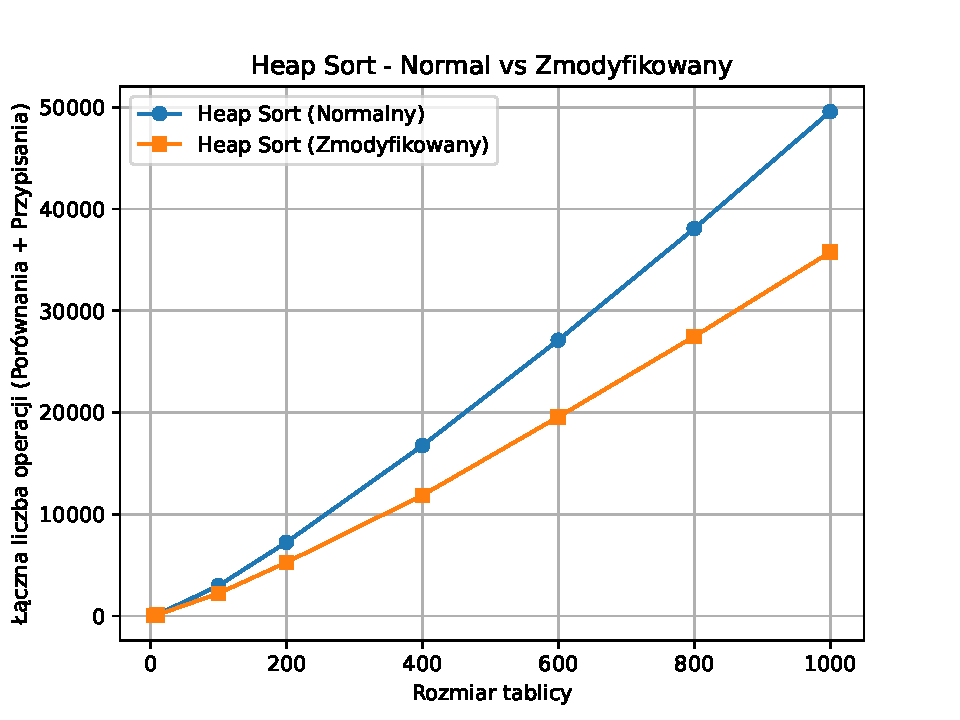
\includegraphics[width=1\textwidth]{Figure_3.pdf}
 \end{figure}
 \item Zarówno klasyczny \texttt{INSERTION\_SORT}, jak i jego modyfikacja są najmniej korzystnym rozwiązaniem.

\begin{figure}[H]
	\centering
	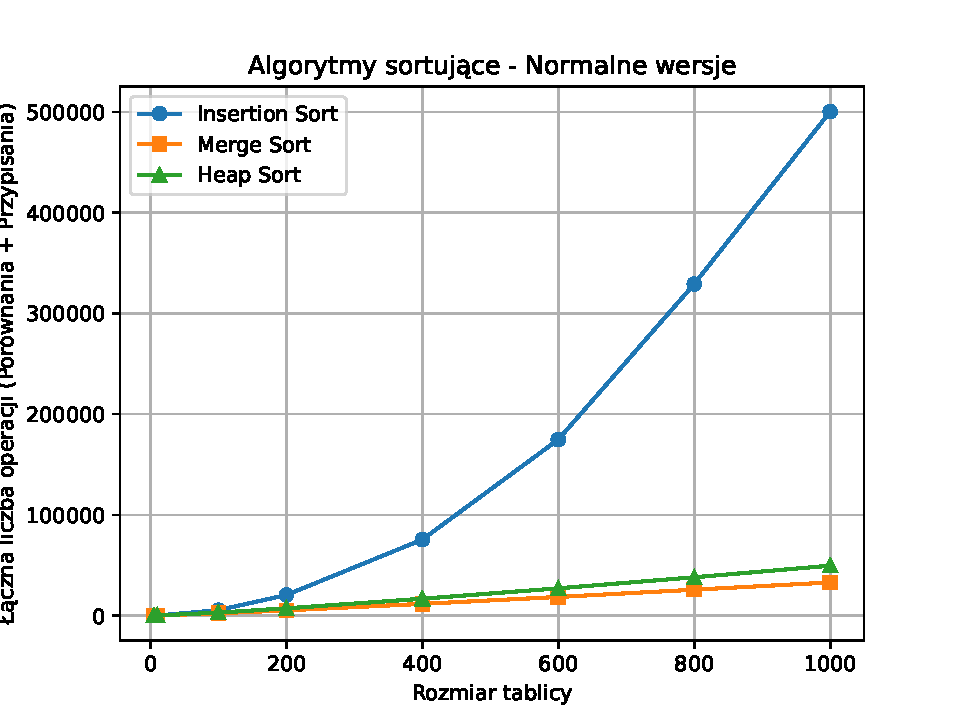
\includegraphics[width=1\textwidth]{Figure_4.pdf}
\end{figure}
\begin{figure}[H]
	\centering
	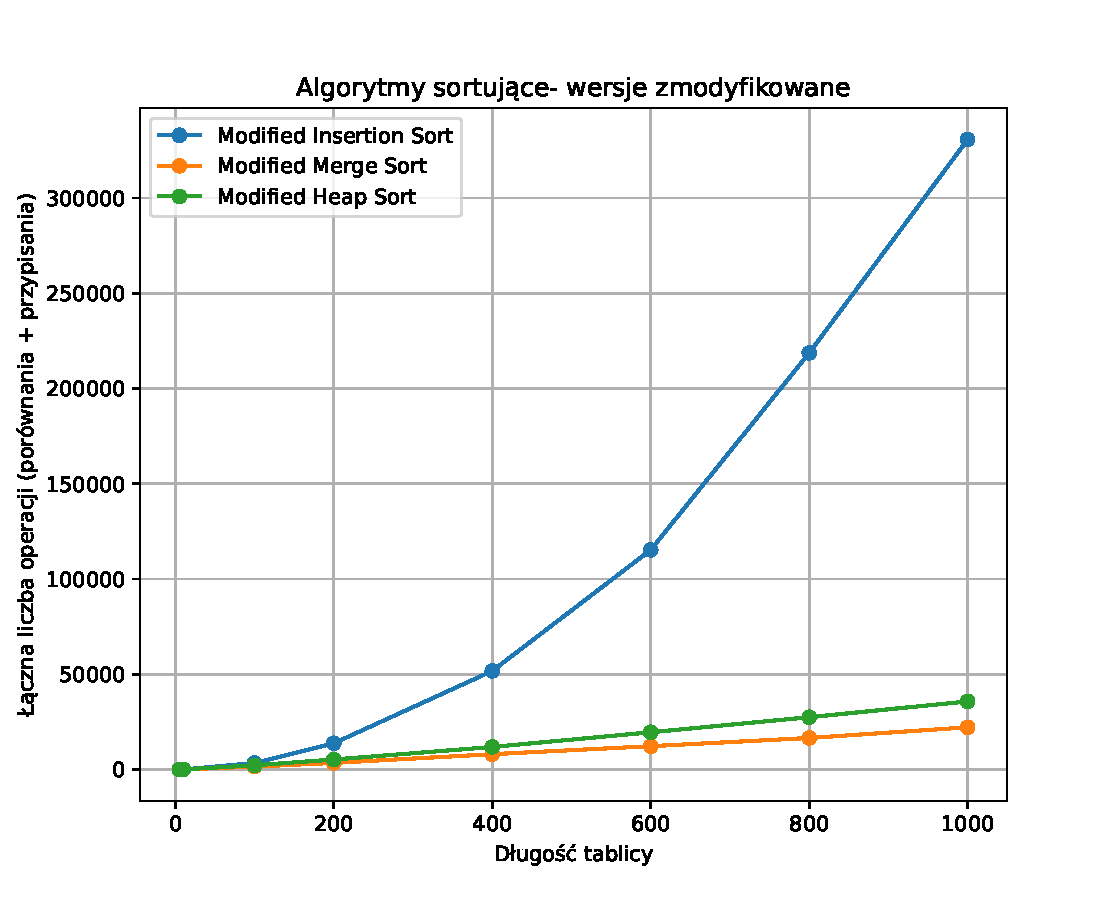
\includegraphics[width=1\textwidth]{Figure_5.1.pdf}
\end{figure}
\end{enumerate}
Poprzez porównanie poprzednio opisanych algorytmów sortujących,  w przypadku danych o dużej objętości lub nieprzewidywalnych zestawów danych, algorytmy \texttt{MERGE\_SORT} i \texttt{HEAP\_SORT} będą bardziej optymalne, podczas gdy \texttt{INSERTION\_SORT} będzie miał sens głównie dla niewielkich zbiorów, lub w pewnej części uporządkowanych.
\end{document}